\begin{figure}
	\begin{center}
		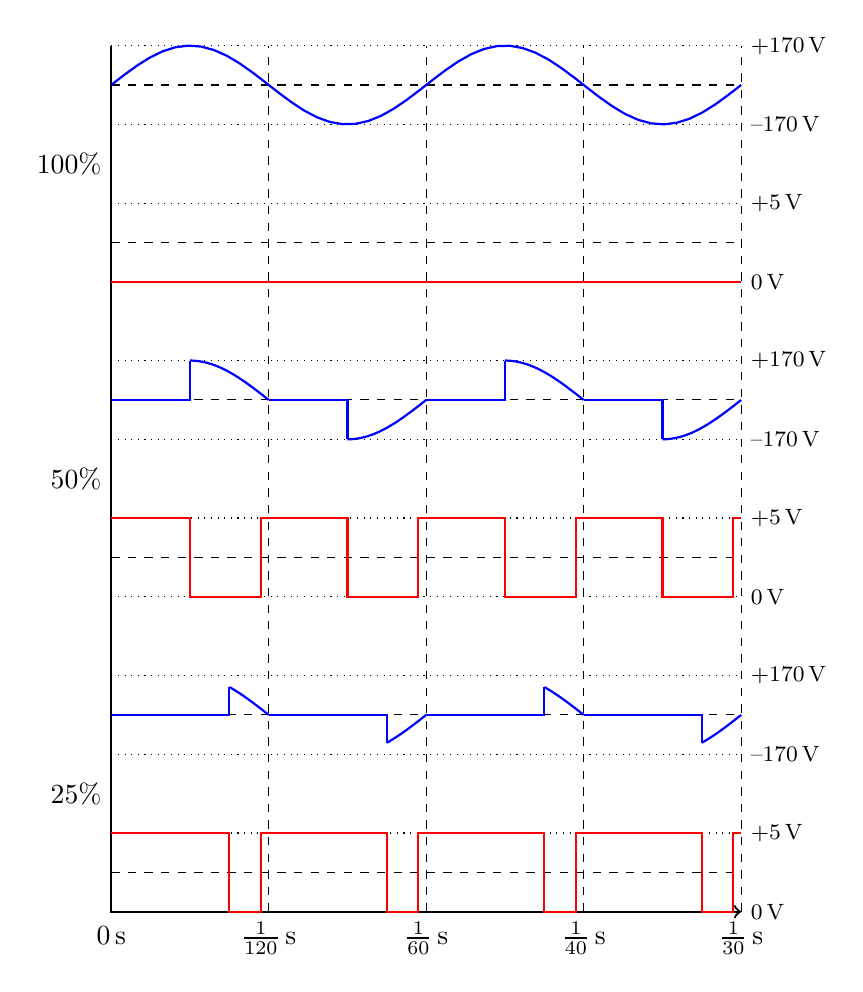
\begin{tikzpicture}[scale=.5]
			\draw [thick, <-] (16,0) -- (0,0) -- (0,22);
			\foreach \x in {4, 8, 12, 16} {
				\draw [dashed] (\x,0) -- (\x,22);
			}
			\foreach \y in {0, 4, 8, 12, 16, 20} {
				\draw [dotted] (0,\y) -- (16,\y);
				\draw [dotted] (0,\y+2) -- (16,\y+2);
				\draw [dashed] (0,\y+1) -- (16,\y+1);
			}
			\foreach \y in {0, 8, 16} {
				\node [right] at (16,\y+2) {\footnotesize +5\,V};
				\node [right] at (16,\y) {\footnotesize 0\,V};
				\node [right] at (16,\y+4) {\footnotesize --170\,V};
				\node [right] at (16,\y+6) {\footnotesize +170\,V};
			}
			\node [left] at (0,3) {25\%};
			\node [left] at (0,11) {50\%};
			\node [left] at (0,19) {100\%};
			\node [below] at (0,0) {\vphantom{$1\over1$}0\,s};
			\node [below] at (4,0) {$1\over120$\,s};
			\node [below] at (8,0) {$1\over60$\,s};
			\node [below] at (12,0) {$1\over40$\,s};
			\node [below] at (16,0) {$1\over30$\,s};

%			\draw [thick,red] (0,2) -- (16,2);
			\draw [thick,red] (0,2) -- (3,2) -- (3,0) -- (3.8,0) -- (3.8,2) --
			          (4,2) -- (7,2) -- (7,0) -- (7.8,0) -- (7.8,2) --
				          (8,2) -- (11,2) -- (11,0) -- (11.8,0) -- (11.8,2) --
				          (12,2) -- (15,2) -- (15,0) -- (15.8,0) -- (15.8,2) --
				 	  (16,2);
			\draw [thick,red] (0,10) -- (2,10) -- (2,8) -- (3.8,8) -- (3.8,10) --
				          (4,10) -- (6,10) -- (6,8) -- (7.8,8) -- (7.8,10) --
				          (8,10) -- (10,10) -- (10,8) -- (11.8,8) -- (11.8,10) --
				          (12,10) -- (14,10) -- (14,8) -- (15.8,8) -- (15.8,10) --
				 	  (16,10);
%			\draw [thick,red] (0,14) -- (1,14) -- (1,12) -- (3.8,12) -- (3.8,14) --
%				          (4,14) -- (5,14) -- (5,12) -- (7.8,12) -- (7.8,14) --
%				          (8,14) -- (9,14) -- (9,12) -- (11.8,12) -- (11.8,14) --
%				          (12,14) -- (13,14) -- (13,12) -- (15.8,12) -- (15.8,14) --
%				 	  (16,14);
			\draw [thick,red] (0,16) -- (16,16);
			\draw [thick,blue] plot[samples=50,domain=0:16](\x,{sin (\x/(4/3.1415926) r)+21});
			\draw [thick,blue] plot[samples=50,domain=2:4](\x,{sin (\x/(4/3.1415926) r)+13});
			\draw [thick,blue] plot[samples=50,domain=6:8](\x,{sin (\x/(4/3.1415926) r)+13});
			\draw [thick,blue] plot[samples=50,domain=10:12](\x,{sin (\x/(4/3.1415926) r)+13});
			\draw [thick,blue] plot[samples=50,domain=14:16](\x,{sin (\x/(4/3.1415926) r)+13});
			\draw [thick,blue] (0,13)--(2,13)--(2,14);
			\draw [thick,blue] (4,13)--(6,13)--(6,12);
			\draw [thick,blue] (8,13)--(10,13)--(10,14);
			\draw [thick,blue] (12,13)--(14,13)--(14,12);
			\draw [thick,blue] plot[samples=50,domain=3:4](\x,{sin (\x/(4/3.1415926) r)+5});
			\draw [thick,blue] plot[samples=50,domain=7:8](\x,{sin (\x/(4/3.1415926) r)+5});
			\draw [thick,blue] plot[samples=50,domain=11:12](\x,{sin (\x/(4/3.1415926) r)+5});
			\draw [thick,blue] plot[samples=50,domain=15:16](\x,{sin (\x/(4/3.1415926) r)+5});
			\draw [thick,blue] (0,5)--(3,5)--(3,5.707106);
			\draw [thick,blue] (4,5)--(7,5)--(7,4.292893);
			\draw [thick,blue] (8,5)--(11,5)--(11,5.707106);
			\draw [thick,blue] (12,5)--(15,5)--(15,4.292893);
		\end{tikzpicture}
		\caption{\label{fig:acdutycycle}Duty Cycles of Logic (red) and AC SSR Outputs (blue)}
	\end{center}
\end{figure}
